% This must be in the first 5 lines to tell arXiv to use pdfLaTeX, which is strongly recommended.
\pdfoutput=1
% In particular, the hyperref package requires pdfLaTeX in order to break URLs across lines.

\documentclass[11pt]{article}

% Remove the "review" option to generate the final version.
\usepackage[]{ACL2023}

% Standard package includes
\usepackage{times}
\usepackage{latexsym}

% For proper rendering and hyphenation of words containing Latin characters (including in bib files)
\usepackage[T1]{fontenc}
% For Vietnamese characters
% \usepackage[T5]{fontenc}
% See https://www.latex-project.org/help/documentation/encguide.pdf for other character sets

% This assumes your files are encoded as UTF8
\usepackage[utf8]{inputenc}

% This is not strictly necessary, and may be commented out.
% However, it will improve the layout of the manuscript,
% and will typically save some space.
\usepackage{microtype}

% This is also not strictly necessary, and may be commented out.
% However, it will improve the aesthetics of text in
% the typewriter font.
\usepackage{inconsolata}

\usepackage[ruled,linesnumbered]{algorithm2e}


\usepackage{graphicx}
\usepackage{subfigure}

\newcommand{\KZ}[1]{\textcolor{blue}{(Kenny: #1)}}
\newcommand{\MY}[1]{\textcolor{orange}{(Mengyue: #1)}}
\newcommand{\XY}[1]{\textcolor{green}{(Xingyuan: #1)}}
\newcommand{\SN}[1]{\textcolor{red}{(Sinong: #1)}}

\newcommand{\secref}[1]{Sec. \ref{#1}}
\newcommand{\figref}[1]{Figure \ref{#1}}
\newcommand{\eqnref}[1]{Eq. (\ref{#1})}
\newcommand{\tabref}[1]{Table \ref{#1}}
\newcommand{\exref}[1]{Example \ref{#1}}

% If the title and author information does not fit in the area allocated, uncomment the following
%
%\setlength\titlebox{<dim>}
%
% and set <dim> to something 5cm or larger.

\title{A Canine Language Lexical Analysis System}

% Author information can be set in various styles:
% For several authors from the same institution:
% \author{Author 1 \and ... \and Author n \\
%         Address line \\ ... \\ Address line}
% if the names do not fit well on one line use
%         Author 1 \\ {\bf Author 2} \\ ... \\ {\bf Author n} \\
% For authors from different institutions:
% \author{Author 1 \\ Address line \\  ... \\ Address line
%         \And  ... \And
%         Author n \\ Address line \\ ... \\ Address line}
% To start a seperate ``row'' of authors use \AND, as in
% \author{Author 1 \\ Address line \\  ... \\ Address line
%         \AND
%         Author 2 \\ Address line \\ ... \\ Address line \And
%         Author 3 \\ Address line \\ ... \\ Address line}

\author{Sinong Wang\textsuperscript{1},
Xingyuan Li\textsuperscript{2}, 
Hridayesh Lekhak\textsuperscript{3},
Mengyue Wu\textsuperscript{4}, Kenny Q. Zhu\textsuperscript{5} \\ \\ 
  \textsuperscript{1,3,5}University of Texas at Arlington, Arlington, Texas, USA \\
  \textsuperscript{2,4}Shanghai Jiao Tong University, Shanghai, China \\
  \texttt{\textsuperscript{1}sxw7663@mavs.uta.edu}\\
  \texttt{\{\textsuperscript{2}xingyuan, \textsuperscript{4}mengyuewu\}@sjtu.edu.cn}\\
  \texttt{\textsuperscript{3}hxl7195@mavs.uta.edu}\\
  \texttt{\textsuperscript{5}kenny.zhu@uta.edu}\\}

\begin{document}
\maketitle

%\begin{abstract}
%  In the age of information explosion, search engines have been an
%  essential tool in people's daily life and query suggestion is one
%  of most useful feature for a standard search engine. However, because
%  most of search engines are keyword-based, many fantastic features would
%  fail when facing concept-based queries, so does query suggestion. In this
%  paper, we propose a framework so that search engines can give acceptable
%  suggestions when facing concept-based queries.
%\end{abstract}

\begin{abstract}
  A class of search queries which contain abstract concepts are studied in
this paper. These queries cannot be correctly interpreted by traditional keyword-based search engines.
  This paper presents a simple framework that detects and instantiates the
abstract concepts by their concrete entities or meanings to produce alternate
queries that yield better search results.
\footnote{Kenny Q. Zhu (corresponding author) is partially
supported by NSFC grants 61100050 and 61033002.}
\end{abstract}


\section{Introduction}

Protein$-$protein interactions (PPIs) are of central importance for the majority of biological functions, such as signal transduction, metabolic pathways, molecular dynamics, and protein networks\cite{Hoffmann.Krallinger.ea:2005}, for they serve as the most fundamental building blocks of the entire interacademic systems of any organisms. Collecting data on pairwise interaction relationships is essential for multiple purpose, including identification of modules with certain functionality\cite{Spirin.Mirny.03}, mapping diseases to dominated genes\cite{Ideker.Sharan.08}, and after all, understanding wholistic metabolic/genetic networks from a system biology perspective.

A lot of databases have been built to store protein and genetic interactions from major model organism species and are available in various standardized formats, such as MINT\cite{Zanzoni.Montecchi-Palazzi.ea:2002}, BIND\cite{Bader.ea:2003}, BIOGRID\cite{DBLP:journals/nar/StarkBRBBT06}, etc. Among those mainstream databases, the data largely rely on voluntary reports by scientists or researchers, besides, comprehensive curation efforts become indispensable for the sake of accuracy. However, the amount of biology-related literatures with respect to protein interactions grows explosively and thus make it either impossible or impractical to manually detect PPI information anymore.

Considering huge amount of PPI information with great wealth hidden in published papers, in recent years, numerous mining techniques have been proposed that aim to extract PPI information automatically from free text, especially machine learning, information retrieval, and natural language processing\cite{DBLP:journals/bib/WinnenburgWPDS08}.These approaches can be roughly categorized into three classes: co$-$occurrence, rule$-$based, and machine learning. 

Co$-$occurrence is the approach with most simplicity and naivete. Just as its name implies, this method intends to find out pairs of proteins that co-occur in the same context. The scope of "same context" ranges from phrase, sentence, paragraph to whole abstract, even document. The underlying assumption is that whenever two proteins are mentioned together by authors, chances are high that there is some kind of relationship between them. However, however, in-context closeness even semantic relation does not necessarily represent actual biological interaction. As a consequence, a large fraction of candidate pairs are mismatched inevitably, causing a high recall but low precision.

The second approach is rule-based extraction, in other words, pattern matching. There are many types of rules, most of them concern natural language processing (NLP). One way is to specify hand-crafted regular expressions before hand, which mostly lean on language usage preference. Besides, by using full or partial (shallow) parsing strategies, more information would be acquired, such as part-of-speech taggers, local dependencies between syntactic components, context-free grammar\cite{DBLP:journals/bioinformatics/TemkinG03}, and full sentence structure. Compared to co$-$occurrence, rule-based approach enjoy better precision but much lower recall. In addition, since the rules are usually derived from training data, that is to say, the improper choice of training data would be significantly lethal, therefore quality of extraction is invariably instable and may not applicable to other data.

The third and most commonly used approach use machine learning techniques, in this case, the task to extract protein$-$protein interactions turns out to be a binary classification problem. Each protein pairs are represented along with a set of features, which is associated with their context, then a well$-$defined classifier gives the answer whether the candidate protein pairs is classified to be qualified PPI. (TO BE FURTHER FILLED!!!)

In this paper, we introduce a general bootstrapping framework for Protein$-$protein interaction extraction from natural text.Our method differs from most of the previous works in three aspects:

(1)The extraction process is driven by only tiny fraction of training data, which are regarded as seed data. In each round, it would derive reliable patterns automatically from seed data, then extract more positive PPI pairs consequently, what's more, the seed data would be augmented by the newly extracted results with high confidence.

(2)multiple graph kernel. 

(3)various evaluation.





%
% File emnlp14-rumor\paper.tex
%
\documentclass[10pt,final,conference,letterpaper]{IEEEtran}
\usepackage{times}
\usepackage{url}
\usepackage{latexsym}
\usepackage{amsmath,algorithm,algpseudocode,caption,subcaption}
\usepackage{epsfig}
\usepackage{graphicx}
\usepackage{booktabs}
\usepackage{color}
\DeclareCaptionType{copyrightbox}
%\setlength\titlebox{6.5cm}    % Expanding the titlebox
\newcommand{\triple}[3]{$\langle$#1, #2, #3$\rangle$}
\newcommand{\pair}[2]{$\langle$#1, #2$\rangle$}
\newcommand{\figref}[1]{Figure \ref{#1}}
\newcommand{\tabref}[1]{Table \ref{#1}}
\newcommand{\secref}[1]{Section \ref{#1}}
%\newcommand{\eqref}[1]{Eq. (\ref{#1})}
\newcommand{\KZ}[1]{\textcolor{blue}{[Kenny: #1]}}
\newcommand{\WK}[1]{\textcolor{red}{[Ke: #1]}}
\newcommand{\ZY}[1]{\textcolor{red}{[Zhiyi: #1]}}

\begin{document}
\title{ExtRA: Automatic Extraction of Review Aspects 
%\Thanks{}
}

\author{
Shi Feng, Kenny Q. Zhu, Zhiyi Luo\\
%Shi Feng$~^{1}$, Kenny Q. Zhu$~^{2}$, Zhiyi Luo$~^{3}$\\
%\vspace{1.6mm}
\fontsize{10}{10}\selectfont\itshape
%Department of Computer Science \& Engineering\\
Shanghai Jiao Tong University, Shanghai, China\\
\vspace{-1cm}
%\fontsize{9}{9}\selectfont\ttfamily\upshape
%$~^{1}$sjtufs@gmail.com, $~^{2}$kzhu@cs.sjtu.edu.cn, 
%$~^{3}$jessieluo1991@gmail.com
}

%\date{\today}
\maketitle
\begin{abstract}
Summarizing users opinions about a product or
service by rating against several distinct and representative aspects
is intuitive and effective. Manual determination of aspects of a product type 
doesn't scale to large and comprehensive e-commerce or consumer review sites
and doesn't adapt to changes in interests.
This paper demonstrates a unsupervised multistage
approach for automatically discovering the best aspect words from massive
amount of textual user reviews of any type of product or service. 
Our experiments showed that the approach is efficient and achieves 
the state-of-the-art accuracies.
\end{abstract}

\section{Introduction}
\label{sec:intro}

Product reviewing is a key character that distinguishes e-commerce 
from conventional retail.
Many websites provides either qualitative or quantitative
summaries of user reviews, organized by important aspects 
of the target product or service.
One example of such \emph{aspect-based review 
summarization}~\cite{hu2004mining} for a hotel on TripAdvisor
as of June 2016 is shown in \figref{fig:tripadvisor}. 
Here, besides the short review passage written by the user, 
the user are asked to give discrete ratings (on the scale of 1-5) 
on various aspects of the hotel room, 
e.g., location and cleanness. The ratings of 
a product from individual reviews can then be aggregated into an overall
ratings of the same product by many users.

\begin{figure}[th]
\centering
\includegraphics[width=0.7\columnwidth]{figures/tripadvisor-short}
\caption{Part of a user review from TripAdvisor.}
\label{fig:tripadvisor}
\end{figure}


Aspect-based review summaries strike a nice middle ground between
detailed text reviews and an all-in-one overall score, yielding
a somewhat balanced view of a product. Such summaries
provide an effective and efficient way of comparing products in
the same category.
%have several advantages compared to the more traditional 
%style of online reviews that consists of a short passage and 
%an overall rating. 
%In aspect-based reviews, more details are provided quantitatively and 
%more directly, and the users can learn about various aspects of a product 
%without having to read the entire review passage. Another advantage of 
%aspect-based reviews is that different products within the same category 
%can be compared directly with respect to multiple aspects, 
%instead of just an overall rating. When researching on products, 
%users spend most of their time comparing different brands and models. 
%Aspect-based review summarization provides an effective and efficient way for 
%doing such comparison, saving the users both time and effort.


%At present, websites that offer aspect-based review summaries typically 
%only feature a single or a small number of product categories, e.g.,
%TripAdvisor.com only features travel related products while Cars.com reviews
%automobiles. 
Because it takes in-depth knowledge to 
characterize a product type using a few keywords that balance between
relevance and diversity, at present, these aspects are primarily hand picked
by the review site operators.
Manual selection of aspects cannot scale to large number of
product types as featured by general e-commerce platforms such as Amazon.com
and Yelp. Moreover, such aspects may change from time to time due to 
evolving user interests.
%These platforms instead turn to automatic review 
%summarization, mined from the user review texts. 

%\begin{figure}[th]
%\centering
%\includegraphics[width=0.8\columnwidth]{figures/phrases}
%\caption{Automatic review summarization for two mobile phones 
%on an e-commerce website}
%\label{fig:phrases}
%\end{figure}
%
%An example of automatic review summarization commonly seen 
%on e-commerce websites is shown in \figref{fig:phrases}. 
%There is a summary of opinion phrases for each phone model, 
%along with the frequency of each phrase mentioned in the 
%reviews. There are two major drawbacks in this form of summarization. 
%First, it is restricted to using the reviews about a specific product. 
%Therefore, summaries are incompatible across different products within 
%the same category - different models may not share the same set of 
%opinion phrases. This makes it less useful for users to compare
%different models.  Second, users' sentiment toward 
%each aspect cannot be quantified and computationally compared - 
%the difference of emotional strength between 
%``extremely good" and ``above average" is hard to capture.
% user cannot choose to express them differently.

%The aspects of a product are supposed to capture the most important features 
%and cover all the facets of the product. The products of the same category 
%share the same set of aspects, however the aspects can be very different 
%across categories. It takes both common knowledge and personal experience 
%with the product to decide which are the appropriate aspects. 
%The websites that can provide aspect-based rating system basically 
%all share a common feature, that is they each focuses on only one or 
%a small range of products. For example TripAdvisor focuses on hotels and 
%Cars.com focuese on cars. The set of aspects is what the consumers base 
%on to compare different products, thus they must be carefully chosen 
%to cover all the facest of the product. Moreoever, at the end of the day 
%the aspects is designed to serve the consumers, especially potential consumers, 
%so they need to reflect what the consumers care about the product. 
%Ideally, the aspects should be decided with user reviews taken into 
%consideration. For a small range of products, the website owner or 
%the retailer may manual designate the set of aspects, 
%however this is intractable for websites like Amazon and TaoBao, 
%which host basically all kinds of products available on the market, 
%and websites like Yelp on which users review thousands of different services. 
%
%Motivated by this observation, we are in need for methods that automatically 
%generate review summarizations. 

Our goal in this paper is to develop an unsupervised system 
for aspect word extraction from a set of user reviews about products within 
the same category.  This problem is similar to topic modeling where aspects 
can be seen as topics, but with a few differences: 
\begin{itemize}
    \item in aspect extraction, we seek to produce 
	aspect words with small mutual semantic overlap; 
    \item aspects may be expressed implicitly through personal experience; and
    \item reviews are a short piece of text, 
	  hence the topics may shift very quickly from 
          sentence to sentence.
\end{itemize}
Previous unsupervised methods for aspect extraction are 
variations of topic models, and cannot capture word semantics and thus
the implicit reference of product aspects. 
In our method we leverage the distributed 
representations of words and sentences. With distributed representations, 
the semantic similarity between two sentences can be more accurately 
calculated without relying too much on the lexical information.
Our proposed method consists 3 clustering steps and
2 ranking phases. The framework achieved state-of-the-art performance 
in end-to-end aspect extraction across multiple domains.

%In \secref{sec:method} we introduce our method step-by-step.
%In \secref{sec:experiments} 
%we evaluate our method on user reviews from multiple domains and demonstrate 
%the effectiveness of our model against other approaches 
%and show how the aspects extracted can be used
%to construct a complete review summarization. 
%In \secref{sec:related}, we discussed
%and compare our work with previous research on aspect-based review 
%summarization.

\section{The System}
\label{sec:method}

The review aspect extraction problem aims to infer $K$ noun 
words from user reviews about the same product type.
Each word represents a distinct aspect or feature of the product type. 
%Here $K$ is an constant parameter for the problem. 
%In unsupervised models for aspect extraction, 
%the set of reviews and the number of aspects are the only inputs.
%Note that in this definition we don't use cross-domain information, 
%that is, for one product type we only use the reviews of that domain.
%This allows us to apply the model to any domain with ease.
%\begin{figure}[th]
%\centering
%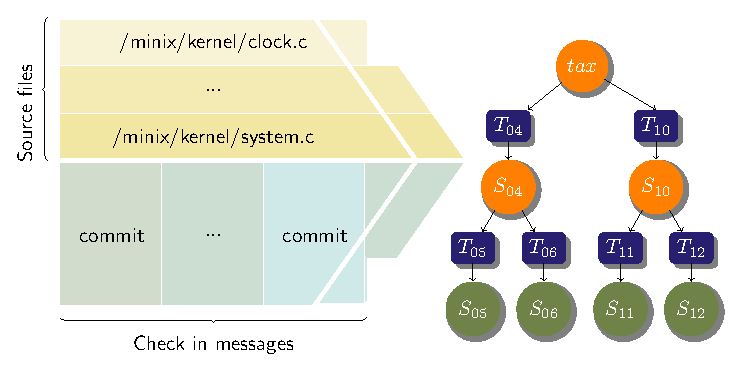
\includegraphics[width=0.9\columnwidth]{figures/framework}
%\caption{Our framework.}
%\label{fig:framework}
%\end{figure}
%
Our system framework consists of 5 steps.
%
%\begin{itemize}
%    \item \textbf{Sentence Clustering}
%
%        We convert each sentence in the reviews into a vector representation 
%        and cluster them in to $N$ clusters of semantically similar sentences.
%
%    \item \textbf{Noise Isolation}
%
%        %As aspects appear as topics in the reviews, 
%        %we use a topic model to infer the potential aspects.
%        To isolate the noises that exist in the sentence cluster,
%	for each sentence cluster we further generate $M$ 
%	topics, resulting in $N\times M$ different word distributions in total.
%
%    \item \textbf{Aspect Inference}
%        
%        We treat each word distribution as a vector and cluster the topics 
%	into $C$ clusters which are the potential aspects. 
%	Here $C$ is purposely set to be larger than $K$. The extra
%	$C-K$ clusters models the redundant aspects.
%        Each cluster contains $N\times M / C$ word distributions, or vectors.
%        We take the mean of these vectors to form $C$ aspect clusters,
%        each being a set of words and their corresponding weights.
%
%    \item \textbf{Cluster Ranking}
%
%        We define a score for the quality of each aspect cluster,
%        and the clusters are ranked by this score.
%
%    \item \textbf{Word Ranking}
%
%        We use WordNet to calculate the semantic distances between the words 
%	in each cluster and adjust the ranking based on the 
%	both the distances and the weights of the words. The top words in each
%	cluster are candidates of the aspect words.
%\end{itemize}
%
%In the following we will explain the motivation and the details of each of
%the five steps. 
%
\subsection{Sentence Clustering}

%One important feature of user reviews is that many topics are 
%compressed into a short paragraph, where each topic corresponds to 
%a potential aspect of the product. 
%A typical hotel review extracted from \figref{fig:tripadvisor} 
%is shown as follows:
%
%\begin{quote}
%Pool is small and only 4 ft but refreshing. Hot tub also there. Staff were super friendly each day. Room was nothing special but clean and comfy. Lots of restaurants and bars nearby. Breakfast was great and despite being a busy weekend there was always a big selection available.
%\end{quote}
%
%In user reviews, topics can shift very quickly.
%Sentences that are close to each other may refer to 
%completely different aspects about the product. Also,
%sentences about the same aspect may not appear in the review consecutively. 
%The existence of such fine-grained semantic shifts in user reviews 
%makes it difficult to apply the the bag-of-word abstraction 
%of normal topic model on reviews.
%Therefore we propose to work on the sentence level instead 
%of the document level, and it would be helpful if we can divide the 
%reviews into topic-oriented segments.
%
%Driven by this observation, in our method the first step is 
%sentence clustering.  For this purpose, 
We represent each sentence in a high-dimensional vector space,
%Instead of using simplistic methods like bag-of-word vector, 
%we leverage a recent development of neural network in natural 
%language processing, the distributed representation.
%In a distributed representation, words and sentences are 
%converted into real-valued vectors.
%The distance of the vectors in the vector space will capture the 
%semantic similarity of the words or sentences.
%In this work we attempt two models, 
using either LSTM (a variant of RNN) or paragraph vector (PV) \cite{le2014distributed}.
%
%\paragraph{Recurrent Neural Network}
%To use RNN for obtaining sentence vectors, 
%we train a neural language model on the review sentences. 
%After the perplexity converges, we use the trained network to 
%process each sentence of the dataset and take the last hidden vector as 
%the vector representation of the sentence. In our method we use a 
%variation of RNN, long-short term memory (LSTM)~\cite{hochreiter1997long} 
%which is reported to have better performance at 
%modeling long sentences \cite{jozefowicz2015empirical}.
%
%\paragraph{Paragraph Vector}
%PV is a simple but powerful extension to Word2vec \cite{mikolov2013distributed} with two components, 
%distributed memory (PV-DM) and distributed bag-of-word (PV-DBOW). 
%The first one is similar to skip-gram in Word2vec and 
%the second is similar to CBOW \cite{mikolov2013distributed}.
%An important advantage of paragraph vector models is that they require 
%no labeled data. Also, it doesn't require human experts to assign weights 
%for words in a paragraph based on linguistic knowledge. 
%The learned vector representations inherit an important property of Word2vec, 
%that is the semantics similarity. Also the final paragraph vector captures the 
%word order information with the part learned from PV-DBOW with the n-gram model.
An advantage of paragraph vector over RNNs is that it can 
leverage trained word vectors, thus requires a smaller training data set. 
%The word vectors can be trained on 
%a much larger corpus so they capture the semantics relationships more 
%accurately.  Consequently, the paragraph vectors can be trained on 
%a relatively small dataset. 
%The performance of paragraph vectors can also be boosted by using pre-trained 
%word vectors that are trained on a larger dataset \cite{mikolov2013linguistic}. 
%%However, previous research show that it is more suitable 
%%to train the word vectors simultaneously for RNNs, 
%%so RNNs cannot leverage the word vectors learned from a larger dataset. 
%Also, the paragraph vector models are simple and 
%don't require the storage of a lot of information. In contrast, for RNN we 
%need to store every state during the forward pass for back-propagation, 
%which is very memory consuming.
%\paragraph{Clustering Sentence Vectors}
We run k-means clustering on the sentence vectors and generate 
$N$ sentence clusters. We then collect the sentences from the same review 
that are clustered together to form smaller fragments of reviews. 
Each original review is divided into several smaller review fragments, 
each belonging to one of the $N$ clusters. As a result, we obtain $N$ 
clusters of review fragments. 

\subsection{Noise Isolation}
There exists noises and overlaps in the clusters formed above.
%The first step, sentence clustering, we might include noise and the sentences 
%within a cluster might not all be about the same aspect. 
%The reason is due to the common occurrences of sentences such as the following
%in the reviews (taken from TripAdvisor):
%
%\begin{quote}
%The room was clean, the staff were friendly, and I would say the price is very reasonable given the proximity to business and leisure destinations around downtown.
%\end{quote}
%
%\begin{quote}
%There is a restaurant just 5 min walk away with nice italian food, pizza was great.
%\end{quote}
%
%In the first sentence multiple aspects are mentioned; in the second sentence, the only aspect is location however lexically it seems to be talking about food.
%With these complicated structures within, 
%it is difficult for RNN or PV to correctly determine the aspects 
%in these sentences. The result is overlaps between clusters about 
%different aspects and noises within each cluster.
%To isolate the noises and resolve such overlap, 
We fix that by applying LDA topic modeling within each sentence cluster, 
treating each review fragment as a document, and generating $M$ smaller topics. 
This will give us in total $N\times M$ topics, or, word distributions. 
%\tabref{table:overlap} shows an example of topics inferred from three
%sentence clusters from hotel reviews and illustrates the overlap problem.
%In this example, five topics were extracted from each sentence cluster, 
%and each row is one topic. It can be seen that the aspects for the 
%three clusters should be {\em room}, {\em location} and {\em price} 
%respectively.
%However, topics shown in boldface font obviously belong to 
%other clusters.  Especially, the last topic of the third cluster 
%appears to be an overlap of more than two clusters.
%The noise isolation step effectively separates the noise topics from other
%topics semantically corehent within a sentence cluster.
%
%\begin{table}[th]
%\centering
%\caption{Topics extracted from three sentence clusters of hotel review.}
%\label{table:overlap}
%\begin{tabular}{|c|l|}
%\hline
%& room bed bedroom size floor \\
%Sentence
%& bedroom room wall size decor \\
%cluster 1
%& room bathroom shower water towel \\
%& room suite size view floor \\
%& room shower area kitchen bed \\\hline
%
%& station minute tube location bus \\
%Sentence
%& location price night place rate\\
%cluster 2
%& location square station street subway\\
%& distance bus subway downtown shopping\\
%& \textbf{restaurant} \textbf{city} \textbf{food} \textbf{buffet} \textbf{place} \\\hline
%
%& price rate service money star\\
%Sentence
%& \textbf{location} \textbf{city} \textbf{star} \textbf{time} \textbf{rate} \\
%cluster 3
%& price service night money city\\
%& price location place night city\\
%& \textbf{location} \textbf{service} \textbf{food} \textbf{price} \textbf{restaurant} \\\hline
%\end{tabular}
%\end{table}


\subsection{Aspect Inference}
\label{sec:topic_clustering}
Each topic is a word distribution, represented by a vector. 
We obtain  more compact representations of those topics by using PCA to 
reduce the topic vectors to 100-dimension.
%We use PCA to reduce the topics vectors to 100-dimension by  
%selecting the 100 words that best distinguish different topics.
Then we perform k-means clustering on the $N\times M$ topics vectors to 
generate $C$ clusters, each containing $(N\times M)/C$ topics.
These are called {\em aspect clusters}.
We set $C$ to be slightly larger than the desired number of product 
aspects $K$, so that the noisy topics can be clustered together and 
later discarded. 
%In an experiment we will evaluate the influence of this redundant clusters on 
%the quality of the final aspects.
%
%\begin{table}[th]
%\caption{Aspect clusters extracted from hotel reviews.
%Each row shows the candidate words of an aspect, sorted by the weight of each word.}
%\label{table:step3}
%\centering
%\begin{tabular}{|l|} \hline
%breakfast, meal, food, tasty, dinner, morning, coffee, tea \\\hline
%room, night, time, bed, day, bathroom, staff, area, place \\\hline
%staff, desk, service, friendly, reception, concierge, helpful \\\hline
%close, city, location, place, central, station, bus, street\\\hline
%bed, shower, spacious, room, size, bathroom, bedroom, floor \\\hline
%price, room, check, night, money, city, location, star, service \\\hline
%location, price, room, night, place, rate, money, time, city  \\\hline
%\end{tabular}
%\end{table}
%
%Finally, for each cluster we take the mean of the $(N\times M)/C$ 
%topics and normalize it
%for the word distribution of that cluster.
%Some example aspect clusters extracted from hotel reviews are 
%shown in \tabref{table:step3}.

\subsection{Cluster Ranking}

We rank the clusters by how ``distinct'' each cluster is from other clusters. 
If a cluster is similar to other clusters, it is considered redundant and of
low quality. We discard $C-K$ least distinct clusters.


%For the $i$th cluster $C_i$ ($i\in [1, C]$), 
%the distinctiveness score $S(i)$ is defined by:
%
%\begin{align}
%S(i) &= \sum_{w\in C_i} S_i(w) \nonumber\\ 
%     &= \sum_{w\in C_i} \log\left(\frac{f_i(w)}{\sum_{j\neq i} f_j(w)}\right)\nonumber \\
%     &= \sum_{w\in C_i}\left[\log f_i(w) - \log\sum_{j\neq c} f_j(a)\right]
%\end{align}
%
%\begin{table}[t]
%\caption{Aspect clusters ranked by distinctiveness score.
%Potential aspect words are boldfaced.}
%\label{table:clustersranked}
%\centering
%\begin{tabular}{|l|} \hline
%\textbf{staff}, desk, \textbf{service}, friendly, reception, concierge, helpful \\\hline
%breakfast, meal, \textbf{food}, tasty, dinner, morning, coffee, tea \\\hline
%\textbf{price}, room, check, night, money, city, location, star, service \\\hline
%bed, shower, spacious, \textbf{room}, size, bathroom, bedroom, floor \\\hline
%close, city, \textbf{location}, place, central, station, bus, street \\\hline
%\textcolor{red}{room, night, time, bed, day, bathroom, staff, area, place} \\\hline
%\textcolor{red}{location, price, room, night, place, rate, money, time, city} \\\hline
%\end{tabular}
%\end{table}
%
\subsection{Word Ranking}
\label{sec:word_ranking}

We rank the words in each cluster 
by considering two factors (similar to TF-IDF): 
the representativeness of the word to the host
cluster; the number of times the word appears in other clusters. 
The most representative word in each cluster
is assumed to be the closest to the centroid of the word cluster.
The distance between two words is the inverse of 
cosine similarity between the word2vec
vectors of the two words.
Then we process the clusters in the order of 
the cluster ranking given in the last step.
When we calculate the score for word $x$ cluster $C_i$,
we also consider the scores of word $x$ in clusters $C_1$ to $C_{i-1}$, 
where the scores have already been calculated. 
We prevent the duplicate aspect words by subtracting the scores 
of $C_1$ to $C_{i-1}$, from the score of $C_i$.
%The score of word $x$ in the $i$th cluster $C_i$ is thus defined by:
%
%\begin{equation}
%s_i(x) = u_i(x) \sum_{y\in C_i}\hat{x}\cdot \hat{y} - \sum_{j=1}^{i-1}s_j(x),
%\label{eq:wordscore}
%\end{equation}
%where $\hat{x}$ is the vector representation of x; $u_i(x)$ is the weight of $x$ in cluster $C_i$.
The words in each cluster is thus ranked by this final score.

\section{Evaluation}
\label{sec:experiments}

We evaluated our framework
against a number of baselines including the state-of-the-art approaches.
%in the end-to-end aspect extraction task.
Our dataset is reviews for 15 categories of product or service crawled from
e-commerce sites such as Amazon.com and Yelp. 
%The review content is plain English text and we do not use any labels 
%for training our model. We use human labels for evaluation. 
%The product categories, their sources and the sizes of the review datasets
%are summarized in \tabref{table:dataset}
%
%\begin{table}[th]
%\centering
%\caption{Dataset summary.} 
%\label{table:dataset}
%\begin{tabular}{|c|c|r|r|}
%\hline
%Product type & Source & No. of Reviews & No. of Words \\ \hline \hline
%hotel        & TripAdvisor & 27145   & 210 \\\hline
%mobile phone & Amazon & 3716    & 136 \\\hline
%mp3 player   & Amazon & 2745    & 128 \\\hline
%laptop       & Amazon & 5471    & 97  \\\hline
%tv           & Amazon & 1237    & 102 \\\hline
%shoes        & Amazon &1748    & 82  \\\hline
%headphone    & Amazon & 1647    & 122 \\\hline
%gps          & Amazon & 1726    & 72  \\\hline
%transportation & Yelp & 3077  & 131 \\\hline
%restaurant   & Yelp & 4016    & 176 \\\hline
%gym          & Yelp & 2481    & 230 \\\hline
%shopping     & Yelp & 2718    & 123 \\\hline
%car dealer   & Yelp & 2839    & 190 \\\hline 
%movie        & Pang et al. \cite{pang2002thumbs} & 3000    & 194 \\\hline
%car          & Cars.com & 1074    & 147 \\\hline
%\end{tabular}
%\end{table}
%
%
%For evaluation, we ask 5 college students proficient with English 
%to annotate ground truth
%aspect words for each product category. For each category, 
%we ask them to provide 5 different words that cover the most important 
%aspects of the corresponding product or service. The labels provided by the
%5 annotators are aggregated together without removing duplicated words, 
%so we have 25 words in total. 
%When evaluating the models, 
%we compare the 5 aspect words generated by the models with those provided 
%by the annotators. 
%We calculate the portion of words among the 25 labels that 
%are correctly generated by the model as the accuracy of the model.
%The ground-truth labels for two product categories are shown 
%in \tabref{table:labels}.
%
%
%\begin{table}[th]
%\centering
%\caption{Labels for hotel and shopping. Each row is provided by one annotator.}
%\label{table:labels}
%\begin{tabular}{|c|l|}
%\hline
%\multirow{5}{*}{hotel}
%& room price location service utility \\
%& room service price food location  \\
%& sleep service room price location  \\
%& location price bedroom bath staff  \\
%& room price bath staff location  \\\hline
%
%\multirow{5}{*}{shopping}
%& location product service price environment \\
%& product price service location ambience \\
%& price food location size facility \\
%& sales location food service environment \\
%& price location service facility food \\\hline
%\end{tabular}
%\end{table}
%
%\subsubsection{Parameter Tuning}
We conduct a few experiments to determine the following
parameter settings: $N=10$, $M=10$, $C=K+2$, i.e. at most two extra clusters.

We compare 5 models in our experiments, 
LDA as a simple baseline, 
D-PLDA \cite{moghaddam2012design} as a representative for joint 
aspect-sentiment models, MG-LDA \cite{titov2008modeling} as 
a representative for aspect extraction topic model,
and two variations of our model LSTM and PV. 
We run the 5 models on the review data of each product type separately. 
For the main experiment, the number of aspects is fixed to 5.

%\begin{figure*}[th]
%\centering
%\includegraphics[width=1.9\columnwidth]{figures/results}
%\caption{Accuracies from different models.}
%\label{fig:results}
%\end{figure*}
%In the end-to-end evaluation, we compare the performance of our models on aspect extraction with three other models as mentioned above. The results are shown in \figref{fig:results}. 
By the accuracy, our two models out-performed all other models in 13 out of 15 
categories. The PV model performs better LSTM, 
which is consistent to our earlier analysis. \tabref{table:hotel_aspect_words}
shows the 5 aspect words by each model for hotel reviews.

\begin{table}[th]
\centering
\small
\caption{Top aspect words for hotels by different models}
\label{table:hotel_aspect_words}
\begin{tabular}{|l|l|} \hline
Ours(PV) & staff, food, price, room, location \\ \hline
Ours(LSTM) & service, location, time, food, bed\\ \hline
MG-LDA & shower, time, food, room, price\\ \hline
DP-LDA & service, station, check, coffee, bed \\ \hline
LDA & stay, location, room, staff, room \\ \hline
\end{tabular}
\end{table}
 
\section{Demo Scenarios}
We present a web demo which depicts the following scenario.
The user logs on and selects
a product type, e.g. ``cell phones'', from a predefined set of categories,  
and sets the number of aspects $K$. 
Then the user clicks the ``generate" button to extract $K$ aspect words for the selected product type.
Upon this, the system computes the review summaries of all cell phones. 
%Upon this, the system shows the $K$ precomputed aspect words for that
%product type, computed from the many user reviews about ``cell phones''. 
%Then the user clicks a button to ``generate review summaries'', which presents
%the review summaries of all cell phones in
%the system. 
Each summary contains the aspects and their scores, computed from the sum of
sentiment scores (1, 0 or -1) against each aspect using LSTM trained on
Stanford Sentiment Treebank~\cite{socher2013recursive}. 
The user may filter out some of the 
results by using the search box (see \figref{fig:summary1}). 
If the user wishes to understand why a product receives a score for a 
certain aspect, they can click on the ``xxx customer reviews'' link
and be directed to the original review snippets with the aspect words and 
sentiment words highlighted. The review snippets by can further grouped by
aspects by clicking on the tabs (see \figref{fig:summary2}). 

\begin{figure}[th]
\includegraphics[width=\columnwidth]{figures/demo1.png}
\caption{Automatically generated 6 aspects for cell phones}
\label{fig:summary1}
\end{figure}

\begin{figure}[th]
\includegraphics[width=\columnwidth]{figures/demo21.png}
\caption{Review snippets displayed by the aspects}
\label{fig:summary2}
\end{figure}


%The second and a minor scenario enables the user to examine the dynamic change
%in aspect words over time for each product type. The system shows a time line,
%annotated with different sets of aspect words, by configurable time periods,
%e.g., every month, 6 months or a year.  
 
\bibliographystyle{IEEEtran}
\bibliography{master}
\end{document}


\section{Approach}
%We first present our methods for testing short circuits in
%models, then modify some of these methods to create
%training data to reverse the short circuit problem
%and enhance the robustness of the models.
% 
%\subsection{Proxy Test for Short Circuit}
%We propose two types of approaches that can be used as proxy test for short circuits.
%One is through inspecting attention maps in
%the models under a white-box setting.
%The other is to generate new test cases by applying different operations on correct choices under a black-box setting.
%
%
%\subsubsection*{White-box Attention Weights~(AW)}
%One intuitive way to detect if an attention-based model is 
%exploiting short circuits is to visualize its attention map. 
%Given a well-trained model and a correctly answered MCQ  in the 
%form of \textit{[CLS] premise [SEP] choice [SEP]}, 
%where \textit{[CLS]} and \textit{[SEP]} are model-dependent 
%delimiters and \textit{choice} refers to the correct choice, 
%we first tokenize the input, feed the token sequence into the model, 
%and extract the attention map of all attention heads from the 
%last encoder layer.
%
%The attention maps are visualized through off-the-shelf tool~\cite{vig-2019-multiscale}
%into user-friendly demo as shown in \figref{fig:att-goodex}. 
%Human annotators are then asked to determine whether there exists 
%strong attention connections from the correct choice to the premise. 
%We consider the MCQ is solved without short-circuiting only if 
%over half of the annotators label it as having strong attention 
%connections. 
%
%Though accurate, such manual annotation is cost-prohibitive to be 
%scaled to larger tests. To remedy this issue, we propose 
%a rule-based procedure to automatically detect the short circuit 
%behavior of a model on MCQ. Specifically, we aggregate the 
%attention maps into one individual map by max-pooling over all 
%attention heads. Then we check if there exists at least one 
%attention score between token in the choice and token in the premise 
%higher than threshold $t_1$ or at least two higher than threshold 
%$t_2$, excluding special tokens like comma and period. 
%We consider that the model not short-circuiting on this MCQ if 
%neither of the two conditions is met. In practice, the 
%threshold $t_1$ and $t_2$ are tuned so as to maximally simulate 
%human annotation. The pseudo-code is shown in Algorithm \ref{AW}.
%
In this section, we first present our methods for testing short circuits in models, and then modify some of these methods to create training data to address the short circuit problem and enhance model robustness.

\subsection{Proxy Test for Short Circuit}
Since no existing method can definitively prove if a model is short-circuiting on a question, we propose two types of approaches that serve as proxy tests for short circuits. These approaches reveal the effects of model short-circuiting, though they can't directly prove the short-circuit itself, similar to dark matter. One approach involves inspecting attention maps in models under a white-box setting, while the other generates new test cases by applying different operations on correct choices under a black-box setting.

\subsubsection*{White-box Attention Weights~(AW)}

One intuitive way to detect if an attention-based model is exploiting short circuits is to visualize its attention map. Given a well-trained model and a correctly answered MCQ in the form of \textit{[CLS] premise [SEP] choice [SEP]}, where \textit{[CLS]} and \textit{[SEP]} are model-dependent delimiters and \textit{choice} refers to the correct choice, we first tokenize the input, feed the token sequence into the model, and extract the attention map of all attention heads from the last encoder layer.

The attention maps are visualized through an off-the-shelf tool~\cite{vig-2019-multiscale} into a user-friendly demo, as shown in \figref{fig:att-goodex}. Human annotators are then asked to determine whether there exists strong attention connections from the correct choice to the premise. We consider the MCQ to be solved without short-circuiting only if over half of the annotators label it as having strong attention connections.

Although accurate, such manual annotation is cost-prohibitive to be scaled to larger tests. To remedy this issue, we propose a rule-based procedure to automatically detect the short circuit behavior of a model on MCQ. Specifically, we aggregate the attention maps into one individual map by max-pooling over all attention heads. Then we check if there exists at least one attention score between a token in the choice and a token in the premise higher than threshold $t_1$, or at least two higher than threshold $t_2$, excluding special tokens like comma and period. We consider the model to not be short-circuiting on this MCQ if neither of the two conditions is met. In practice, the thresholds $t_1$ and $t_2$ are tuned to maximally simulate human annotation. The pseudo-code is shown in Algorithm \ref{AW}.


\begin{algorithm}
\small
	\caption{Attention Weight Thresholding}
	\label{AW}
\hspace*{0.02in} {\bf Input:} 
premise $P$, correct choice $C$, model $M$,  threshold $t_1$ and $t_2$. \\
\hspace*{0.02in} {\bf Output:}
binary 0/1 label $L$.
	\begin{algorithmic}[1]
		\State initialize counters $c_1$ and $c_2$ to 0.
		\State tokenize the formatted input as sequence of tokens $S$.
		\State feed $S$ into $M$ and extract the last layer's attention maps $Attn_{all}$.
		\State aggregate $Attn_{all}$ into $Attn_{max}$ by max-pooling over all attention heads.
		\For{$w_1$ in $C$}
		\For{$w_2$ in $P$}
		\If{$Attn_{max}(w_1, w_2)> t_1$}
				$c_1$ += 1
		\EndIf
		\If{$Attn_{max}(w_1, w_2) > t_2$}
				$c_2$ += 1
		\EndIf
		\EndFor
		\EndFor
		\State output 1 if $c_1>0$ or $c_2\geq 2$ and 0 otherwise.
	\end{algorithmic}
\end{algorithm}

\subsubsection*{Black-box Choice Operator}
\label{sec:proxy}
While attention-based testing methods can detect short circuits within the encoder directly, they don't directly detect short circuits in the end-to-end MCQ model, which also includes a linear layer above the attention-based pretrained language model. Additionally, these methods are limited to a family of models with inherent attention mechanisms.

A more desirable approach is an automatic end-to-end black-box test that is model-independent. In black-box testing, if a model correctly answers an MCQ, we slightly modify the MCQ by applying a certain``operation'' on the original correct choice to produce another wrong choice. The newly generated MCQ must share the same correct choice as the original question. By observing the model's response to the second MCQ, we can infer whether the model short-circuits on the original MCQ.If the model still selects the correct choice, then we consider it to have passed the test and not short-circuited on the original MCQ. The challenge now is how to construct the new wrong choice by implementing the operation in various ways.

In this paper, we consider the operations listed in \tabref{table:proxyop}. Some of the operations were mentioned in previous literature, while others are proposed here (marked with *).
The first line in each cell describes the operation, and the next two lines provide an example of constructing a false choice from a choice in the original question. An operation may either preserve (p) the truth value (\crosssymbol $\rightarrow$ \crosssymbol) or change (c) the truth value of the choice (\checksymbol $\rightarrow$ \crosssymbol).

\begin{table}[th]
        \centering
        \scriptsize
        \begin{tabular}{l|l}
                \toprule
                \textbf{Oper.} &\textbf{Description and Example}\\
                \hline
                \multirow{3}{*}{Neg+} & Add negation (c) \\
                & \textit{They called the police to come to my house. \checksymbol} \\
                & \textit{They {\color{olive}{didn't}}  called the police to come to my house. \crosssymbol} \\
                \hline
                \multirow{3}{*}{Neg-} &Remove negation (c) \\
                & \textit{Ben {\color{olive} never} starts working out. \checksymbol} \\
                & \textit{Ben starts working out. \crosssymbol}\\
                \hline

                \multirow{3}{*}{NER} &Randomly replace person names (c)\\
                 & \textit{A big wave knocked {\color{olive} Mary} down . \checksymbol} \\
                & \textit{A big wave knocked {\color{olive} Kia} down . \crosssymbol} \\
                \hline
                \multirow{3}{*}{PR*} & Switch pronoun by gender or quantity (c)\\
        &\textit{{\color{olive} She} had a great time .\checksymbol} \\
        &\textit{{\color{olive} He} had a great time . \crosssymbol} \\
                \hline
                \multirow{3}{*}{PI*} &Instantiate pronoun by randome person (c) \\
        &\textit{{\color{olive} They} gave Tom a new latte with less ice . \checksymbol}\\
        &\textit{{\color{olive} Nathanael} gave Tom a new latte with less ice . \crosssymbol}\\
                \bottomrule
%               \hline
                \multirow{3}{*}{Adv} &Add adverbs for emphasis (c) \\
                &\textit{The ocean was a calm as a bathtub .\crosssymbol} \\
                &\textit{{\color{olive} In fact} the ocean was a calm as a bathtub .\crosssymbol} \\
                \hline
               \multirow{3}{*}{CO*} & Crossover: Swap the true choices between two questions (p)\\ 
	&\textit{\color{olive}Josh got sick . \checksymbol} \\
	&\textit{\color{olive}{She had a great time .\crosssymbol}}  \\
\hline
                \multirow{3}{*}{Syn} &Replace adj/adv with synonym (p) \\
                &\textit{Dawn felt {\color{olive} happy} about getting away with it . \crosssymbol} \\
                &\textit{Dawn felt {\color{olive} glad} about getting away with it . \crosssymbol} \\

		\bottomrule
               \multirow{3}{*}{MT*} & Mutate: Swap two consecutive words (c) \\
		& \textit{Deb said yes {\color{olive} to} {\color{olive} Tim} 's marriage proposal. \crosssymbol} \\
		& \textit{Deb said yes {\color{olive} Tim} {\color{olive} to} 's marriage proposal .\crosssymbol} \\
               \hline
\multirow{3}{*}{Voice} &Swap subject and object (c) \\
        & \textit{{\color{olive}{Kara}} asked {\color{olive}{the neighbors}}  not to litter in their yard . \checksymbol} \\
        &\textit{{\color{olive}{the neighbors}} asked  {\color{olive}{Kara}}  not to litter in their yard . \crosssymbol}\\
                \bottomrule
        \end{tabular}
        \caption{A number of operations considered for proxy testing. 
First line in each cell describes the operation, the next two lines
give an example of how to construct a false choice from a choice of
the original question. An operation may either 
preserve (p) the truth value (\checksymbol $\rightarrow$ \checksymbol, \crosssymbol $\rightarrow$ \crosssymbol) or change (c) the truth value of
the choice (\checksymbol $\rightarrow$ \crosssymbol).  }
        \label{table:proxyop}
\end{table}

Inspired by boundary testing in software engineering, we can classify these operations into three equivalent classes (three vertical sections in \tabref{table:proxyop}), depending on the nature of the \textit{false} choice constructed:
\begin{enumerate}
\item The syntax and semantics are correct, and the \textit{false} choice appears similar to the \textit{true} choice.
\item The syntax and semantics are correct, and the \textit{false} choice appears distinct from the \textit{true} choice.
\item Either syntax or semantics is incorrect.
\end{enumerate}

The last class is not suitable for testing short circuits because the model may answer the proxy question correctly by eliminating the false choice due to errors in it, not by considering the premise.

We focus on perturbations on negation~\cite{checklist2020acl}, NER~\cite{checklist2020acl}, and pronouns in the first class and adverbial~\cite{wsp2020acl}, crossover, and synonym~\cite{checklist2020acl,wsp2020acl} in the second class.

While most of the operations are self-explanatory, the \textit{crossover} operation is unique and deserves special attention. Inspired by molecular biology, for each MCQ in the dataset that the model answers correctly, we substitute the original false choice with the true choice from another randomly sampled MCQ. The substituted choice remains false in the proxy question. The operation can be visually explained in \figref{fig:cross}.

\begin{figure}[th]
\centering
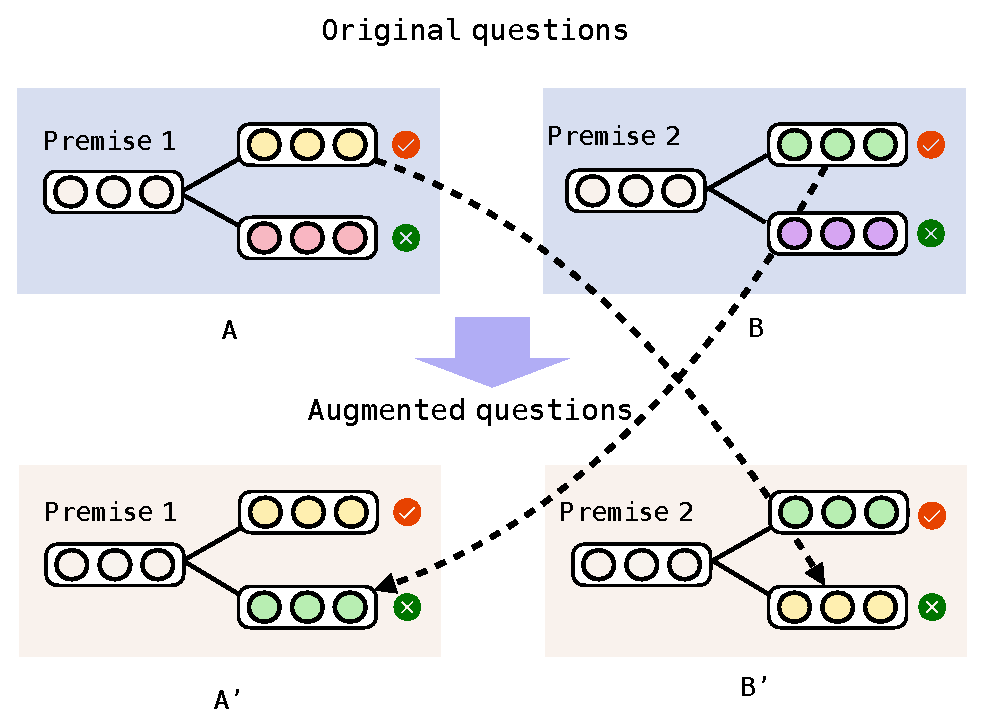
\includegraphics[width=\columnwidth]{figure/cross.eps}
\caption{The Crossover Operation: the true choice of both questions
are used to replace the false choices of these questions to create
two new proxy questions.}
\label{fig:cross}
\end{figure}

Compared to all other operations in classes 1 and 2, the crossover provides a proxy question that is most different from the original one but easier from a human perspective. This is because the two choices may be quite unrelated. If the model does not handle it correctly, it may be more indicative of a short circuit. As a result, the crossover is potentially a better short circuit test than others.

Another advantage of the crossover operation is that we can generate multiple false choices for an original question at a low cost, allowing us to test each original question more thoroughly. In contrast, most other operations cannot produce an adequate number of different variants of the original choice.

In summary, the proposed black-box choice operator provides a more generalizable and model-independent method for detecting short circuits in MCQ models. By applying various operations to create proxy questions, we can assess the model's performance and robustness more accurately, contributing to the development of better and more reliable models in the future.

\subsection{Improving Model Robustness by Data Augmentation}

If a model is shown to short-circuit by the proxy tests, its performance may decline, especially when applied to out-of-domain test data. To make models more robust, one natural thought is to generate more data to encourage models to focus on the relation between the premise and choices. While the operations used to generate proxy tests can also be utilized for data augmentation, not all of them are scalable or able to generate enough data for training.

The two operations that can generate a substantial amount of data are crossover and mutation. These operations can be applied to the training data to enhance the model's robustness.

\subsubsection*{Crossover for Data Augmentation}

Crossover is a good option for data augmentation because the two choices were originally true answers in their respective questions and presumably carry spurious features if the model was short-circuiting. By incorporating crossover into the training data, the model is forced to consider the premise in order to determine which choice is better.

\subsubsection*{Mutation for Data Augmentation}

Mutation has two flavors: (1) swap the words only in the true choice; (2) swap the words both in the true and the false choice. Compared to crossover, mutation has the potential to be more effective at improving model robustness. It not only forces the model to look into the premise due to its two very similar choices (same set of tokens), but also makes the model more sensitive to fine differences in word orders and enhances the model's prior grammatical knowledge.

\subsubsection*{Differentiating between Proxy Test and Data Augmentation}

It is essential to differentiate between the use of crossover and mutation operations in proxy tests and data augmentation. In proxy tests, these operations are used to modify the test data to assess the model's short-circuiting behavior. In contrast, when applied for data augmentation, the same operations work on the training data to enhance the model's robustness and generalization capabilities.

In conclusion, data augmentation through crossover and mutation operations can contribute to improving model robustness by encouraging models to focus on the relationship between the premise and choices. By incorporating these operations into the training data, models are forced to consider the premise and become more sensitive to the fine differences in word orders, leading to better performance and reliability in real-world applications.


\section{EXPERIMENT EVALUATION}
In this section, we conduct extensive experiments to evaluate the effect of our proposed solution to derive causality knowledge. All the experiments are implemented in Python and run on a Intel Xeon 32 CPU(2.60GHz) with 173GB memory.


\subsection{Dataset}
The dataset crawled from financial news website \footnote{ \url { http://finance.sina.com.cn }} contains \textbf{4 991 000} articles, and there are \textbf{111 330 205} sentences. The number of unique sentences is \textbf{75 572 053}, occupied  \textbf{67.88\%} of the total sentences. The number of sentence with casual cue words is \textbf{7 147 141}, occupied \textbf{9.46\%}.

\textbf{Causal Pattern statistic.} The elaborate casual patterns can be grouped into 6 groups of templates, each containing pattern in one group  has the same meaning but different words. The matched sentences distribution over these groups of patterns is shown in Fig.\ref{tab3}. from which, we can find the first three take most proportion of the whole sentences. and we will use these three kind of sentence to carry on later experiments.
\begin{table*}[t]
	\caption{Number of sentences extracted by causal patterns}
	\begin{center}
		\begin{tabular}{|c|c|c|c|}
			\hline
			\textbf{Pattern template}& \textbf{Pattern}& \textbf{Number}& \textbf{Rate}\\
			\hline
			A->B&因为 A,B&2000242&0.4831573605311576\\
			\hline
			A->B&A,所以 B&1530311&0.4831573605311576\\
			\hline
			A->B&因为 A, 所以B&2000242&0.3696457846359572\\
			\hline
			$A_1,A_2->B$&因为 $A_1$, 且 $A_2$, 所以 B&22356&0.005400079566389746\\
			\hline
			$A->B_1,B_2$&因为 A,所以 $B_1$ 且 $B_2$&10178&0.002458490330413081\\
			\hline
			$A_1,A_2->B_1,B_2$&因为 $A_1$, 且 $A_2$,所以 $B_1$  且 $B_2$&1&2.415494527817922e-07\\
			\hline
		\end{tabular}
		\label{tab3}
	\end{center}
\end{table*}	


\textbf{Our newly built Knowledge Base.}
TODO: explaination
\begin{table}[t]
	\caption{Knowledge Base}
	\begin{center}
		\begin{tabular}{|c|c|}
			\hline
			\textbf{Name}&\textbf{Number}\\
			\hline
			IsA pairs (Taxonomy)&515163\\
			\hline
			Concepts (Taxonomy)&81082\\
			\hline
			instances (Taxonomy)&158693\\
			\hline
			Common Sense Pairs&7316977\\
			\hline
		\end{tabular}
		\label{tab3}
	\end{center}
\end{table}	

\textbf{Rule.}
some numbers of the rule instances, candidate instances and final rules are show in \ref{tab3}.
\begin{table}[t]
	\caption{Rule number}
	\begin{center}
		\begin{tabular}{|c|c|}
			\hline
			\textbf{Name}&\textbf{Number}\\
			\hline
			Rule Instances&??\\
			\hline
			Candidate Rules&??\\
			\hline
			Relation Number&??\\
			\hline
		\end{tabular}
		\label{tab3}
	\end{center}
\end{table}	

\subsection{Case Study}

Here we show some rules derived, some are good\ref{fig:good_rule_case}, some are bad \ref{fig:bad_rule_case}. Also, We would do some error analysis.
\subsubsection{Good Cases}
\begin{figure}[htbp]
	\centerline{\includegraphics[width=0.9\columnwidth]{figures/good_rule_case}}
	\caption{Good Cases.}
	\label{fig:good_rule_case}
\end{figure}	
	TODO: explanation   
	
\subsubsection{Bad Cases}
\begin{figure}[htbp]
	\centerline{\includegraphics[width=0.9\columnwidth]{figures/bad_rule_case}}
	\caption{Bad Cases.}
	\label{fig:bad_rule_case}

\end{figure}
	TODO: explanation why they are bad
	




\subsection{Rule instantiation}
Rule instantiation also called Rule deduction is shown in \ref{fig:instantiation}
\begin{figure}[htbp]
	\centerline{\includegraphics[width=0.9\columnwidth]{figures/instantiation}}
	\caption{Rule Instantiation .}
	\label{fig:instantiation}
\end{figure}

%\textit{Question Answer}
%\textit{Make decision}








\section{Conclusion}
We implement a novel sequence-based dependency parsing
framework which takes advantage of high order features 
in parsing history. 
%We can also adapt beam search to this framework so as to
%relax the strictly greedy nature. Vine pruning\cite{rush2012vine} could
%be incorporated to speed up the parsing.
More importantly, we discovered that the parsing accuracy is very sensitive to
the quality of parsing sequence. Future work can be focused on
developing better sequence predictors that outperform Malt action classifier.
Furthermore, we use two sets of features for sequence predictor and
head mapper right now. A unified set of features between these two components
are worth exploring.
%Besides, better sequence predicting method and unified feature
%representation of two components are worth exploring.
%
%Though we currently get a not bad result,
%the sequence predictor still needs more exploration.
%According to our experiment, slightly changes
%on the sequence can lead to a fatal decline on accuracy. Ensuring the match degree of training sequence and testing
%sequence demands a high quality of sequence predictor.
%
%Further, the features in our current implementation are not expanded and well tuned yet  and we are free to define high order features to make use of parsing history. Our framework is flexible to merge other technics to enhance the performance. Introducing beam could make up for our greedy decoder and improve our accuracy. Vine pruning\cite{rush2012vine} could speed up parsing process. Besides, better sequence predicting method and unified feature representation of two components are worth exploring.



\section*{Limitations}

Despite the audio denoising process, our final canine sound sentences still contain some noise. This portion of noise was labeled as 14 noise phonemes during the phoneme labeling process. Moreover, due to the lack of ground truth for canine sound phonemes or vocabulary, we could only evaluate the transcription results from acoustic perspectives.








%\section*{Ethics Statement}
%
%\section*{Acknowledgements}


% Entries for the entire Anthology, followed by custom entries
%\bibliography{anthology,custom}
\bibliography{references}
\bibliographystyle{acl_natbib}



\end{document}
